% QuizForge Backend Documentation - Part 4: Security & API
\documentclass[12pt,a4paper]{report}

% Packages
\usepackage[utf8]{inputenc}
\usepackage[T1]{fontenc}
\usepackage{geometry}
\usepackage{graphicx}
\usepackage{tikz}
\usetikzlibrary{shapes.multipart, positioning, arrows.meta, calc}
\usepackage{listings}
\usepackage{xcolor}
\usepackage{hyperref}
\usepackage{tcolorbox}
\usepackage{fancyhdr}
\usepackage{titlesec}
\usepackage{longtable}
\usepackage{array}
\usepackage{booktabs}
\usepackage{enumitem}
\usepackage{pdflscape}

% Page geometry
\geometry{
    a4paper,
    left=25mm,
    right=25mm,
    top=30mm,
    bottom=30mm
}

% Colors
\definecolor{codegreen}{rgb}{0,0.6,0}
\definecolor{codegray}{rgb}{0.5,0.5,0.5}
\definecolor{codepurple}{rgb}{0.58,0,0.82}
\definecolor{backcolour}{rgb}{0.95,0.95,0.92}
\definecolor{javakey}{rgb}{0.5,0,0.35}

% Code listing style
\lstdefinestyle{javastyle}{
    backgroundcolor=\color{backcolour},
    commentstyle=\color{codegreen},
    keywordstyle=\color{javakey}\bfseries,
    numberstyle=\tiny\color{codegray},
    stringstyle=\color{codepurple},
    basicstyle=\ttfamily\footnotesize,
    breakatwhitespace=false,
    breaklines=true,
    captionpos=b,
    keepspaces=true,
    numbers=left,
    numbersep=5pt,
    showspaces=false,
    showstringspaces=false,
    showtabs=false,
    tabsize=2,
    frame=single,
    language=Java
}

\lstset{style=javastyle}

% Hyperref setup
\hypersetup{
    colorlinks=true,
    linkcolor=blue,
    filecolor=magenta,
    urlcolor=cyan,
    pdftitle={QuizForge Backend Documentation - Part 4},
    pdfauthor={System Documentation},
    pdfsubject={Security and API Documentation},
}

% Headers and footers
\pagestyle{fancy}
\fancyhf{}
\fancyhead[L]{\leftmark}
\fancyhead[R]{QuizForge Backend - Part 4}
\fancyfoot[C]{\thepage}

% Title formatting
\titleformat{\chapter}[display]
{\normalfont\huge\bfseries}{\chaptertitlename\ \thechapter}{20pt}{\Huge}

% Document metadata
\title{%
    \Huge\textbf{QuizForge} \\
    \Large Complete Backend Documentation \\
    \large Part 4: Security \& API Documentation \\
    \normalsize Version 1.0.0
}
\author{Technical Documentation}
\date{\today}

\begin{document}

% Title page
\maketitle
\tableofcontents
\newpage

% Include chapters for Part 4
% Chapter 7: Security
\chapter{Security Layer}

\section{Overview}

The security layer implements JWT-based authentication and role-based authorization using Spring Security 6.x (Spring Boot 3.2.0).

\section{SecurityConfig}

\subsection{Complete Source Code}

\begin{lstlisting}[caption=SecurityConfig.java]
@Configuration
@EnableWebSecurity
@EnableMethodSecurity
public class SecurityConfig {

    @Autowired
    private JwtRequestFilter jwtRequestFilter;

    @Value(''${cors.allowed-origins}'')
    private String allowedOrigins;

    @Bean
    public SecurityFilterChain securityFilterChain(
            HttpSecurity http) throws Exception {
        http
            .cors(cors -> cors.configurationSource(
                corsConfigurationSource()))
            .csrf(csrf -> csrf.disable())
            .authorizeHttpRequests(auth -> auth
                .requestMatchers(''/api/auth/**'').permitAll()
                .requestMatchers(''/swagger-ui/**'', 
                    ''/v3/api-docs/**'', 
                    ''/swagger-ui.html'').permitAll()
                .requestMatchers(''/api/admin/**'').hasRole(''ADMIN'')
                .requestMatchers(''/api/candidate/**'')
                    .hasRole(''CANDIDATE'')
                .anyRequest().authenticated()
            )
            .sessionManagement(session -> session
                .sessionCreationPolicy(SessionCreationPolicy.STATELESS))
            .addFilterBefore(jwtRequestFilter, 
                UsernamePasswordAuthenticationFilter.class);

        return http.build();
    }

    @Bean
    public CorsConfigurationSource corsConfigurationSource() {
        CorsConfiguration configuration = new CorsConfiguration();
        configuration.setAllowedOrigins(
            List.of(allowedOrigins.split('','')));
        configuration.setAllowedMethods(
            Arrays.asList(''GET'', ''POST'', ''PUT'', ''DELETE'', ''OPTIONS''));
        configuration.setAllowedHeaders(Arrays.asList(''*''));
        configuration.setAllowCredentials(true);
        
        UrlBasedCorsConfigurationSource source = 
            new UrlBasedCorsConfigurationSource();
        source.registerCorsConfiguration(''/**'', configuration);
        return source;
    }

    @Bean
    public PasswordEncoder passwordEncoder() {
        return new BCryptPasswordEncoder();
    }
}
\end{lstlisting}

\subsection{Line-by-Line Explanation}

\begin{itemize}[leftmargin=*]
    \item \textbf{@Configuration}: Marks as Spring configuration class
    \item \textbf{@EnableWebSecurity}: Enables Spring Security
    \item \textbf{@EnableMethodSecurity}: Enables method-level security annotations
    
    \item \textbf{SecurityFilterChain Bean}
    \begin{itemize}
        \item Configures HTTP security using lambda DSL (Spring Security 6.x style)
        \item Replaces deprecated \texttt{WebSecurityConfigurerAdapter}
    \end{itemize}
    
    \item \textbf{CORS Configuration}
    \begin{itemize}
        \item Enables Cross-Origin Resource Sharing
        \item References custom configuration source
    \end{itemize}
    
    \item \textbf{CSRF Disabled}
    \begin{itemize}
        \item Cross-Site Request Forgery protection disabled
        \item Safe for stateless JWT authentication
        \item Required for REST APIs
    \end{itemize}
    
    \item \textbf{Authorization Rules}
    \begin{itemize}
        \item \texttt{/api/auth/**}: Public (login endpoint)
        \item \texttt{/swagger-ui/**}: Public (API documentation)
        \item \texttt{/api/admin/**}: Requires ADMIN role
        \item \texttt{/api/candidate/**}: Requires CANDIDATE role
        \item All other requests: Authenticated users only
    \end{itemize}
    
    \item \textbf{Session Management}
    \begin{itemize}
        \item \texttt{STATELESS}: No HTTP sessions created
        \item Each request authenticated independently via JWT
        \item Enables horizontal scalability
    \end{itemize}
    
    \item \textbf{JWT Filter}
    \begin{itemize}
        \item Added before \texttt{UsernamePasswordAuthenticationFilter}
        \item Processes JWT token from Authorization header
        \item Sets authentication in SecurityContext
    \end{itemize}
    
    \item \textbf{CORS Configuration Source}
    \begin{itemize}
        \item Reads allowed origins from properties
        \item Supports multiple origins (comma-separated)
        \item Allows all HTTP methods needed for REST
        \item Allows credentials (cookies, auth headers)
    \end{itemize}
    
    \item \textbf{PasswordEncoder Bean}
    \begin{itemize}
        \item BCrypt algorithm for password hashing
        \item Automatically salted
        \item Adjustable strength factor
    \end{itemize}
\end{itemize}

\section{JwtUtil}

\subsection{Purpose}
Utility class for JWT token generation, parsing, and validation using JJWT library.

\subsection{Key Methods}

\begin{lstlisting}[caption=JWT Token Generation]
public String generateToken(String email, String role) {
    Map<String, Object> claims = new HashMap<>();
    claims.put(''role'', role);
    return createToken(claims, email);
}

private String createToken(Map<String, Object> claims, 
                          String subject) {
    return Jwts.builder()
            .setClaims(claims)
            .setSubject(subject)
            .setIssuedAt(new Date(System.currentTimeMillis()))
            .setExpiration(new Date(System.currentTimeMillis() 
                + expiration))
            .signWith(getSigningKey(), SignatureAlgorithm.HS512)
            .compact();
}
\end{lstlisting}

\textbf{Token Structure:}
\begin{itemize}
    \item \textbf{Claims:} Custom data (role)
    \item \textbf{Subject:} User email
    \item \textbf{Issued At:} Token creation time
    \item \textbf{Expiration:} Configurable (24 hours default)
    \item \textbf{Signature:} HMAC-SHA512 algorithm
\end{itemize}

\begin{lstlisting}[caption=JWT Token Extraction]
public String extractEmail(String token) {
    return extractClaims(token).getSubject();
}

public String extractRole(String token) {
    return extractClaims(token).get(''role'', String.class);
}

private Claims extractClaims(String token) {
    return Jwts.parserBuilder()
            .setSigningKey(getSigningKey())
            .build()
            .parseClaimsJws(token)
            .getBody();
}
\end{lstlisting}

\begin{lstlisting}[caption=JWT Token Validation]
public Boolean isTokenValid(String token) {
    try {
        Jwts.parserBuilder()
                .setSigningKey(getSigningKey())
                .build()
                .parseClaimsJws(token);
        return !isTokenExpired(token);
    } catch (Exception e) {
        return false;
    }
}

public Boolean isTokenExpired(String token) {
    return extractExpiration(token).before(new Date());
}
\end{lstlisting}

\textbf{Validation Checks:}
\begin{itemize}
    \item Signature verification
    \item Expiration check
    \item Format validation
    \item Exception handling for malformed tokens
\end{itemize}

\section{JwtRequestFilter}

\subsection{Purpose}
Filter that intercepts every request to extract and validate JWT tokens, setting authentication context.

\subsection{Complete doFilterInternal Method}

\begin{lstlisting}[caption=JWT Request Filter Logic]
@Override
protected void doFilterInternal(HttpServletRequest request, 
                               HttpServletResponse response, 
                               FilterChain chain)
        throws ServletException, IOException {

    final String authorizationHeader = 
        request.getHeader(''Authorization'');

    String email = null;
    String jwt = null;

    if (authorizationHeader != null && 
        authorizationHeader.startsWith(''Bearer '')) {
        jwt = authorizationHeader.substring(7);
        
        try {
            if (!jwtUtil.isTokenValid(jwt)) {
                response.setStatus(
                    HttpServletResponse.SC_UNAUTHORIZED);
                response.setContentType(''application/json'');
                response.getWriter().write(
                    ''{\''error\'': \''Invalid or expired token\''}'');
                return;
            }
            
            email = jwtUtil.extractEmail(jwt);
            String role = jwtUtil.extractRole(jwt);

            if (email != null && SecurityContextHolder
                    .getContext().getAuthentication() == null) {
                UsernamePasswordAuthenticationToken authToken = 
                    new UsernamePasswordAuthenticationToken(
                        email, null, Collections.singletonList(
                            new SimpleGrantedAuthority(
                                ''ROLE_'' + role)));
                authToken.setDetails(
                    new WebAuthenticationDetailsSource()
                        .buildDetails(request));
                SecurityContextHolder.getContext()
                    .setAuthentication(authToken);
            }
        } catch (Exception e) {
            logger.error(''JWT validation failed: '' + e.getMessage());
            response.setStatus(HttpServletResponse.SC_UNAUTHORIZED);
            response.setContentType(''application/json'');
            response.getWriter().write(
                ''{\''error\'': \''Invalid token: '' + 
                e.getMessage() + ''\''}'');
            return;
        }
    }

    chain.doFilter(request, response);
}
\end{lstlisting}

\subsection{Processing Flow}

\begin{enumerate}
    \item Extract Authorization header
    \item Check for ''Bearer '' prefix
    \item Extract JWT token (remove ''Bearer '' prefix)
    \item Validate token signature and expiration
    \item If invalid, return 401 Unauthorized and stop
    \item Extract email and role from token
    \item Create \texttt{UsernamePasswordAuthenticationToken}
    \item Add role as \texttt{SimpleGrantedAuthority} with ''ROLE\_'' prefix
    \item Set authentication in \texttt{SecurityContext}
    \item Continue filter chain
\end{enumerate}

\subsection{Security Context}

\textbf{Authentication Object Contents:}
\begin{itemize}
    \item \textbf{Principal:} User email (username)
    \item \textbf{Credentials:} null (JWT is stateless)
    \item \textbf{Authorities:} List with single role (ROLE\_ADMIN or ROLE\_CANDIDATE)
    \item \textbf{Details:} Request details (IP, session ID, etc.)
\end{itemize}

\section{Authentication Flow Diagram}

\begin{figure}[h]
\centering
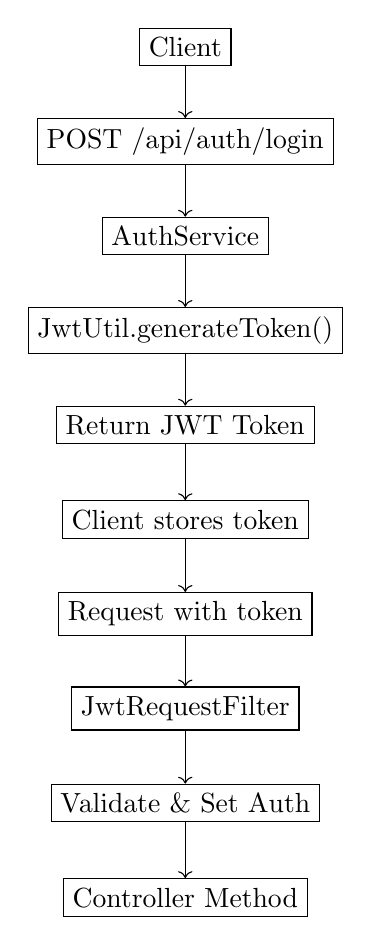
\begin{tikzpicture}[node distance=1.2cm]
    \node[draw, rectangle] (client) {Client};
    \node[draw, rectangle, below of=client] (login) {POST /api/auth/login};
    \node[draw, rectangle, below of=login] (authservice) {AuthService};
    \node[draw, rectangle, below of=authservice] (jwtutil) {JwtUtil.generateToken()};
    \node[draw, rectangle, below of=jwtutil] (response) {Return JWT Token};
    \node[draw, rectangle, below of=response] (store) {Client stores token};
    \node[draw, rectangle, below of=store] (request) {Request with token};
    \node[draw, rectangle, below of=request] (filter) {JwtRequestFilter};
    \node[draw, rectangle, below of=filter] (validate) {Validate \& Set Auth};
    \node[draw, rectangle, below of=validate] (controller) {Controller Method};
    
    \draw[->] (client) -- (login);
    \draw[->] (login) -- (authservice);
    \draw[->] (authservice) -- (jwtutil);
    \draw[->] (jwtutil) -- (response);
    \draw[->] (response) -- (store);
    \draw[->] (store) -- (request);
    \draw[->] (request) -- (filter);
    \draw[->] (filter) -- (validate);
    \draw[->] (validate) -- (controller);
\end{tikzpicture}
\caption{Complete Authentication Flow}
\end{figure}

\section{JWT Token Example}

\subsection{Token Structure}

A JWT consists of three parts separated by dots:

\texttt{header.payload.signature}

\textbf{Header (Base64):}
\begin{lstlisting}[language=json]
{
  ''alg'': ''HS512'',
  ''typ'': ''JWT''
}
\end{lstlisting}

\textbf{Payload (Base64):}
\begin{lstlisting}[language=json]
{
  ''role'': ''ADMIN'',
  ''sub'': ''admin@quizforge.com'',
  ''iat'': 1699632000,
  ''exp'': 1699718400
}
\end{lstlisting}

\textbf{Signature:}
\begin{lstlisting}
HMACSHA512(
  base64UrlEncode(header) + ''.'' + base64UrlEncode(payload),
  secret
)
\end{lstlisting}


% Chapter 8: API Documentation
\chapter{OpenAPI 3.0 Documentation}

\section{OpenAPI Configuration}

\subsection{OpenApiConfig Class}

\begin{lstlisting}[caption=OpenApiConfig.java]
@Configuration
public class OpenApiConfig {

    @Bean
    public OpenAPI customOpenAPI() {
        return new OpenAPI()
                .info(new Info()
                        .title(''QuizForge API'')
                        .version(''1.0'')
                        .description(''Online Quiz Platform - Role-based API (ADMIN & CANDIDATE)''))
                .servers(List.of(new Server()
                    .url(''http://localhost:8080'')
                    .description(''Development Server'')))
                .addSecurityItem(new SecurityRequirement()
                    .addList(''bearerAuth''))
                .components(new Components()
                        .addSecuritySchemes(''bearerAuth'',
                                new SecurityScheme()
                                        .type(SecurityScheme.Type.HTTP)
                                        .scheme(''bearer'')
                                        .bearerFormat(''JWT'')
                                        .description(''Enter JWT token obtained from /api/auth/login'')));
    }
}
\end{lstlisting}

\subsection{Configuration Elements}

\begin{itemize}
    \item \textbf{Info:} API metadata (title, version, description)
    \item \textbf{Servers:} Available server endpoints
    \item \textbf{SecurityRequirement:} Global security requirement
    \item \textbf{SecurityScheme:} JWT Bearer authentication definition
\end{itemize}

\section{API Endpoints Reference}

\subsection{Authentication Endpoints}

\begin{longtable}{|p{3cm}|p{10cm}|}
\hline
\textbf{Endpoint} & POST /api/auth/login \\
\hline
\textbf{Summary} & Login and get JWT token \\
\hline
\textbf{Description} & Use admin@quizforge.com for ADMIN role, any other email for CANDIDATE role \\
\hline
\textbf{Request Body} & \begin{lstlisting}[language=json]
{
  ''email'': ''string'',
  ''password'': ''string''
}
\end{lstlisting} \\
\hline
\textbf{Response 200} & \begin{lstlisting}[language=json]
{
  ''token'': ''string'',
  ''email'': ''string'',
  ''name'': ''string'',
  ''role'': ''string''
}
\end{lstlisting} \\
\hline
\textbf{Security} & None (public endpoint) \\
\hline
\caption{Login Endpoint Documentation}
\end{longtable}

\subsection{Admin Endpoints}

\subsubsection{GET /api/admin/quizzes}

\begin{longtable}{|p{3cm}|p{10cm}|}
\hline
\textbf{Summary} & Get all quizzes \\
\hline
\textbf{Description} & Retrieve list of all quizzes \\
\hline
\textbf{Security} & Bearer JWT (ADMIN role required) \\
\hline
\textbf{Response 200} & Array of QuizSummaryResponse \\
\hline
\textbf{Response Example} & \begin{lstlisting}[language=json]
[
  {
    ''id'': 1,
    ''title'': ''Java Basics'',
    ''description'': ''Test your Java knowledge'',
    ''duration'': 30,
    ''isActive'': true,
    ''createdBy'': ''Admin User'',
    ''createdAt'': ''2024-11-10T10:00:00'',
    ''questionCount'': 10
  }
]
\end{lstlisting} \\
\hline
\caption{Get All Quizzes Documentation}
\end{longtable}

\subsubsection{GET /api/admin/quizzes/\{id\}}

\begin{longtable}{|p{3cm}|p{10cm}|}
\hline
\textbf{Summary} & Get quiz by ID \\
\hline
\textbf{Parameters} & id (path, required): Quiz ID \\
\hline
\textbf{Security} & Bearer JWT (ADMIN role) \\
\hline
\textbf{Response 200} & QuizResponse with full details \\
\hline
\textbf{Response 404} & Quiz not found \\
\hline
\caption{Get Quiz by ID Documentation}
\end{longtable}

\subsubsection{POST /api/admin/quizzes}

\begin{longtable}{|p{3cm}|p{10cm}|}
\hline
\textbf{Summary} & Create new quiz \\
\hline
\textbf{Request Body} & \begin{lstlisting}[language=json, basicstyle=\ttfamily\tiny]
{
  ''title'': ''Java Basics'',
  ''description'': ''Test your Java knowledge'',
  ''duration'': 30,
  ''isActive'': true,
  ''questions'': [
    {
      ''questionText'': ''What is Java?'',
      ''type'': ''MULTIPLE_CHOICE'',
      ''points'': 1,
      ''options'': [
        {
          ''optionText'': ''Programming language'',
          ''isCorrect'': true
        },
        {
          ''optionText'': ''Coffee brand'',
          ''isCorrect'': false
        }
      ]
    }
  ]
}
\end{lstlisting} \\
\hline
\textbf{Response 201} & Created quiz with assigned IDs \\
\hline
\textbf{Response 400} & Validation errors \\
\hline
\caption{Create Quiz Documentation}
\end{longtable}

\subsubsection{PUT /api/admin/quizzes/\{id\}}

\begin{longtable}{|p{3cm}|p{10cm}|}
\hline
\textbf{Summary} & Update existing quiz \\
\hline
\textbf{Parameters} & id (path, required): Quiz ID \\
\hline
\textbf{Request Body} & Same as POST (full quiz data) \\
\hline
\textbf{Response 200} & Updated quiz \\
\hline
\textbf{Response 404} & Quiz not found \\
\hline
\caption{Update Quiz Documentation}
\end{longtable}

\subsubsection{DELETE /api/admin/quizzes/\{id\}}

\begin{longtable}{|p{3cm}|p{10cm}|}
\hline
\textbf{Summary} & Delete quiz \\
\hline
\textbf{Parameters} & id (path, required): Quiz ID \\
\hline
\textbf{Response 204} & No content (success) \\
\hline
\textbf{Response 404} & Quiz not found \\
\hline
\caption{Delete Quiz Documentation}
\end{longtable}

\subsubsection{GET /api/admin/quizzes/\{id\}/analytics}

\begin{longtable}{|p{3cm}|p{10cm}|}
\hline
\textbf{Summary} & Get quiz analytics \\
\hline
\textbf{Parameters} & id (path, required): Quiz ID \\
\hline
\textbf{Response 200} & \begin{lstlisting}[language=json]
{
  ''quizId'': 1,
  ''quizTitle'': ''Java Basics'',
  ''totalAttempts'': 15,
  ''averageScore'': 7.5,
  ''highestScore'': 10,
  ''lowestScore'': 3
}
\end{lstlisting} \\
\hline
\caption{Quiz Analytics Documentation}
\end{longtable}

\subsection{Candidate Endpoints}

\subsubsection{GET /api/candidate/quizzes}

\begin{longtable}{|p{3cm}|p{10cm}|}
\hline
\textbf{Summary} & Get available quizzes \\
\hline
\textbf{Security} & Bearer JWT (CANDIDATE role) \\
\hline
\textbf{Response 200} & Array of active quizzes (summary) \\
\hline
\caption{Get Available Quizzes Documentation}
\end{longtable}

\subsubsection{POST /api/candidate/quizzes/\{quizId\}/start}

\begin{longtable}{|p{3cm}|p{10cm}|}
\hline
\textbf{Summary} & Start quiz attempt \\
\hline
\textbf{Parameters} & quizId (path, required) \\
\hline
\textbf{Response 200} & \begin{lstlisting}[language=json]
{
  ''id'': 1,
  ''quizId'': 1,
  ''quizTitle'': ''Java Basics'',
  ''startedAt'': ''2024-11-10T10:00:00'',
  ''submittedAt'': null,
  ''score'': null,
  ''totalPoints'': 10,
  ''status'': ''IN_PROGRESS''
}
\end{lstlisting} \\
\hline
\caption{Start Quiz Documentation}
\end{longtable}

\subsubsection{GET /api/candidate/quizzes/\{quizId\}}

\begin{longtable}{|p{3cm}|p{10cm}|}
\hline
\textbf{Summary} & Get quiz questions \\
\hline
\textbf{Description} & Returns questions with options, but isCorrect is hidden \\
\hline
\textbf{Parameters} & quizId (path, required) \\
\hline
\textbf{Response 200} & QuizResponse (without correct answers) \\
\hline
\caption{Get Quiz Questions Documentation}
\end{longtable}

\subsubsection{POST /api/candidate/quizzes/submit}

\begin{longtable}{|p{3cm}|p{10cm}|}
\hline
\textbf{Summary} & Submit quiz answers \\
\hline
\textbf{Request Body} & \begin{lstlisting}[language=json]
{
  ''attemptId'': 1,
  ''answers'': [
    {
      ''questionId'': 1,
      ''selectedOptionId'': 3,
      ''textAnswer'': null
    },
    {
      ''questionId'': 2,
      ''selectedOptionId'': null,
      ''textAnswer'': ''Sample answer''
    }
  ]
}
\end{lstlisting} \\
\hline
\textbf{Response 200} & AttemptResponse with calculated score \\
\hline
\caption{Submit Quiz Documentation}
\end{longtable}

\subsubsection{GET /api/candidate/quizzes/my-attempts}

\begin{longtable}{|p{3cm}|p{10cm}|}
\hline
\textbf{Summary} & Get my quiz attempts \\
\hline
\textbf{Response 200} & Array of user's attempts with scores \\
\hline
\caption{Get My Attempts Documentation}
\end{longtable}

\subsubsection{GET /api/candidate/quizzes/attempts/\{attemptId\}}

\begin{longtable}{|p{3cm}|p{10cm}|}
\hline
\textbf{Summary} & Get attempt result \\
\hline
\textbf{Parameters} & attemptId (path, required) \\
\hline
\textbf{Response 200} & Detailed attempt results \\
\hline
\textbf{Response 403} & Not your attempt (forbidden) \\
\hline
\caption{Get Attempt Result Documentation}
\end{longtable}

\section{Swagger UI Access}

The interactive API documentation is available at:

\texttt{http://localhost:8080/swagger-ui.html}

Features:
\begin{itemize}
    \item Try API endpoints directly from browser
    \item Automatic request/response examples
    \item JWT authentication support
    \item Grouped by controller tags
    \item Alphabetically sorted operations
\end{itemize}

\section{OpenAPI JSON Specification}

The raw OpenAPI 3.0 specification is available at:

\texttt{http://localhost:8080/v3/api-docs}

Can be used with:
\begin{itemize}
    \item Code generators (OpenAPI Generator)
    \item API testing tools (Postman, Insomnia)
    \item Documentation generators
    \item Mock server tools
\end{itemize}



\end{document}
